% !TeX root = ../../thesis.tex

\section{Neither Secure Boot nor Bitlocker}

% premise of attack
The first attack is performed without enabling any additional security mechanisms (e.g. Secure Boot, BitLocker).

\subsection{Bootkit}

% general concept
deviate the boot flow
access to the hard drive from the UEFI Environment
deploy payload so that it is executed

% UEFI does not support NTFS
Windows uses NTFS formatting for its primary file system \cite{microsoft-ntfs-overview}, thus we need to use an NTFS driver to access the Windows installation.
% windows uses NTFS
The UEFI specification mandates compliant firmware to support FAT12, FAT16 and FAT32 \cite[13.3.1.1]{uefi-spec}, since this does not include NTFS edk2 does not come with an NTFS driver.

% search for UEFI NTFS driver with write access
% open source fork of ntfs-3g for UEFI
Luckily open source NTFS drivers are readily available such as ntfs-3g from tuxera \cite{ntfs-3g} which allow for read and write access, on top of that there already exists a port to UEFI created by pbatard \cite{ntfs-3g-uefi}.

% compile
% spits out .efi file
We can compile this driver with edk2 following the listed steps and receive a .efi executable file.

% try in EFI shell
% what is the EFI shell
\TODO{better summary of UEFI shell}
Part of the UEFI specifications is a shell specification which is a feature rich UEFI shell application to interact with the UEFI environment.
% https://docstore.mik.ua/manuals/hp-ux/en/5991-1247B/ch04s13.html
\TODO{better listing of capabilities}
It offers commands for
boot,
configuration,
device, driver, handle
filesystem
network
memory
scripting.
For now driver loading and filesystem navigation are of relevance.

% how to use uefi shell
\TODO{look up official guideline to booting into console}
% we are trying in qemu where the shell is available in boot options
% real hardware might require the uefi shell application .efi from the user via usb stick
The UEFI shell can be part of the boot options or requires the user to supply the executable via a removable medium such as a USB stick.

% explain shell screen
Upon invocation, the shell application performs an initialization during which it \TODO{does what? whats important for us here} and produces output that is equivalent to the output of the execution of the commands \lstinline{ver} and \lstinline{map -terse} \cite[3.3 Initialization]{uefi-shell}. \lstinline{ver} displays the version of the UEFI specification the firmware conforms to \cite[5.3 Shell Commands]{uefi-shell}.

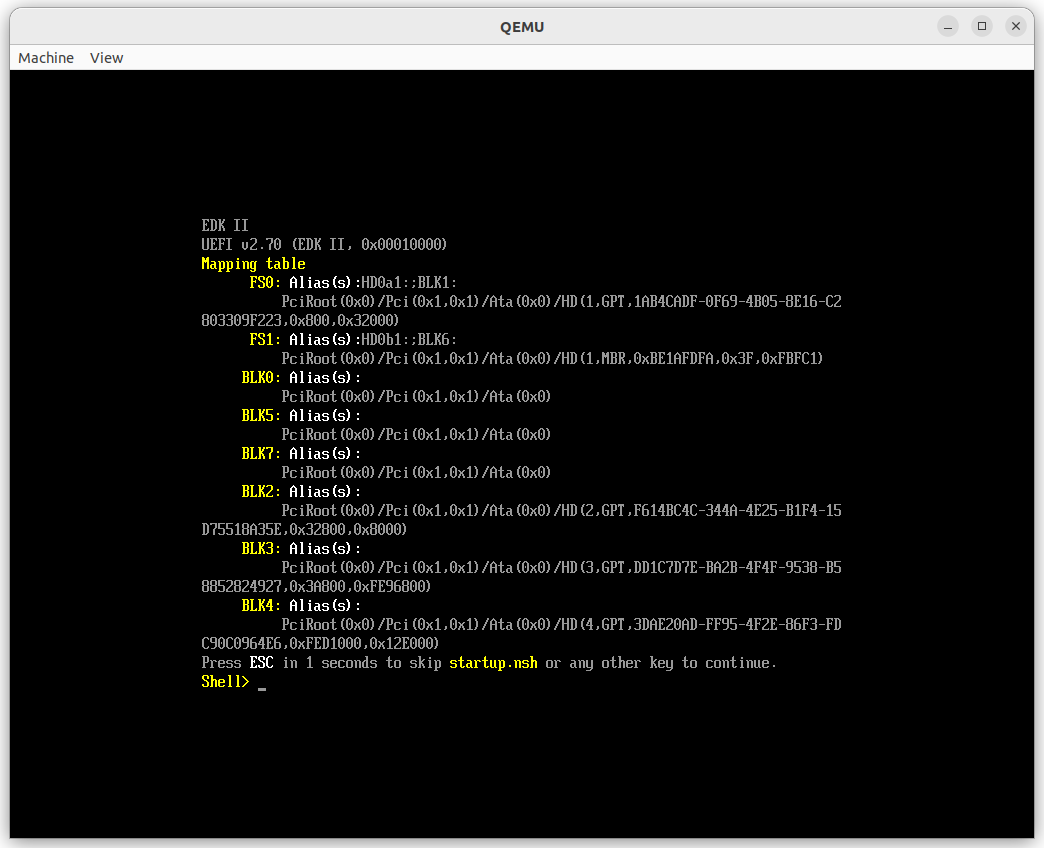
\includegraphics[width=\textwidth]{attacks/neither/01_uefi_shell.png}


% showing mapping, also available with map command
% consistent device mapping, comparable to partition names in windows
The map command is very interesting for file access with the shell, it displays a mapping table between user defined alias names and device handles. The aliases can be used instead of a device path when submitting commands via the command line interface. The UEFI shell also produces default mappings, notably for file systems \cite[3.7.2. Mappings]{uefi-shell}. These mappings are designed to be consistent across reboots as long as the hardware configuration stays the same, they are comparable to Windows partition letters. \cite[Appendix A]{uefi-shell}

% blk and fs
\cite[13.3.2 Partition Disocvery]{uefi-spec}
\TODO{find in spec what precise mapping mechanism}
When we inspect the mapping table we can see FSx and BLKx aliases, FSx maps to file systems and BLKx to block devices. This identification is performed via instances of the Simple File System Protocol and \TODO{double check} Block I/O Protocol which present the interfaces to access the devices they are installed to.
% explain Simple File System Protocol
\TODO{explain file system indepent abstraction better}
\TODO{explain block devices}
The Simple File System Protocol \cite[13.4 Simple File System Protocol]{uefi-spec} provides, together with the File Protocol, file-type access to the device it is installed on. The two protocols are independent of the underlying file system the media is formatted with.
\TODO{UEFI supported file systems}
By default UEFI supports FAT32

Drivers providing these protocols use the Block I/O Protocol to access the underlying media.


% load NtfsDxe.efi
Our NTFS UEFI Driver is one such abstraction and needs to be loaded now, this is done by first entering the alias, for the file system containing the NtfsDxe.efi, followed by a colon.
\TODO{alias for fs eingeben was macht das}
This effectively switches the console's working directory to be the root of the entered file system, now we caninvoke load with the path to the executable. The output indicates whether loading the driver was successful.
% drivers
% We can now list
\TODO{maybe better command here}
With the command drivers, we can list all currently loaded drivers and some basic information about them, such as number of devices managed. We can see that the NTFS driver already manages devices.

% map -r "reset all the default mappings in a system this option is useful if the system configuration has changed since the last boot"
% new mapping and fs ontop of old blk
\TODO{reword maybe move the block device stuff up}
We can now reset all default mappings with the map -r command to receive an updated list including the file system now provided by the NTFS driver. The mapping also shows us that the file system now sits on top of a device which previously was only listed as a block device indicating that the NTFS driver uses this block-wise access to offer the Simple File System Protocol.

As done before we now type the alias of the new file system followed with a colon to switch to NTFS formatted file system. With ls we can list the current directory's content and confirm by the presence of the Windows folder that we are on the volume containing the Windows installation.


% navigate to Windows folder
% means read works
% try creating folder to test write
\TODO{Windows file access privileges}
We now navigate into the Windows folder to test whether we have unrestricted read and write access, since is not the case if done by an unprivileged user when performed from within Windows. Accessing folders and viewing their contents is possible but creation of a new folder fails.

% debug why it failed
% find out its from windows having hibernation enabled by default
% change source code to not fallback to read only when encountering hibernation file
Upon debugging the NTFS driver it appears to be that the drivers falls back to read only when it encounters a file that indicates that the Windows system is in hibernation mode. Windows seems to have hibernation enabled by default and as such our rootkit should not rely on it being disabled, we can change the code of the NTFS driver to not fallback when encountering this file.

We now know that provided we get to load the NTFS driver we can access a Windows installation and subsequently the entire data of unencrypted hard drives. Since our rootkit will not use the UEFI shell we need to have the NTFS driver load as part of the boot process.
% try to package in firmware image instead of loading from external medium
We can put the NTFS driver into the DXE Volume where the DXE Dispatcher of the DXE Core will automatically try to load it.

% for hardware use spi clamp to  dump image
For this, we have to read out the firmware image, modify the contents and write the new image back to hardware. This can be done by using a spi flash programmer and clamping the physical chip.
% for qemu we can build it ourselves
If we want to use emulation we can build the Open Virtual Machine Firmware (OVMF) Package from edk2 which is a firmware image for virtual machines.

% we can open image with UEFITool
Now that we have the image we can edit it with UEFITool, which is an editor for firmware images conforming to the UEFI PI spec \cite{uefitool}.
In UEFITool we navigate to the DXE Volume containing the DXE Core and DXE drivers.
% remove previous NTFS driver if present, for full control, might be read only etc
% in UEFITool search for string
Before adding our driver we remove any other NTFS driver packed in the image by OEMs, because they might be read only or otherwise restricted and would inhibit our NTFS driver from controlling a device. UEFITool offers a search through the entire firmware image. We can search for "NTFS" as a case insenstive string, since most drivers either have a User Interface Section which contains a human-readable name for tools like UEFITool\cite[Vol 3, 3.2.5]{pi-spec} or support the optional Component Name Protocol which is part of the UEFI Driver Model and returns the name of a driver \cite[11.5]{uefi-spec}. If this would not suffice it would be possible to search for the NTFS magic number indicating that a volume is formatted with NTFS, this number is ascii encoded NTFS followed by four white spaces.

% since files are part of file sections we cant drop in the .efi
If we now want to add our NTFS driver .efi file with UEFITool we notice that it is displayed as having an unknown subtype, this is because added a file without file sections, a DXE driver has three mandatory sections: PE32 executable, version and DEPEX section \cite[Vol 3, 2.1.4.1.4]{pi-spec}.
% compile dxe driver within ovmf
% generate unused volume to receive .ffs file with version, depex, user interface and pe section
For these files to be generated it is easiest to simply build the NTFS driver as part of the edk2 OVMF and have it packaged in a firmware volume. This can be an unused volume or for debugging purposes the DXE volume, for real hardware we can use the output of the build process which is a .ffs file. The .ffs file contains the PE32, version, DEPEX and an optional user interface section.
% add in NTFS driver .ffs file
% on hardware use write access with clamp
% qemu just use path to modified image
We can now simply insert the .ffs file into the target firmware image with UEFITool and overwrite the SPI flash with modified image by using the programmer again.

% now upon opening uefi shell
% we instantly see the filesystem
If we now boot up the UEFI shell the splash screen immediately lists the NTFS formatted device in the mapping table indicating that the driver was successfully loaded during DXE dispatch.

% access to all drivers etc
\TODO{why did we choose dxe stage}

% try to use ntfs-driver in code
% this is our first rootkit iteration
% payload will also be DXE driver
% package payload in firmware image
The next step is to now use theblo NTFS driver programmatically by writing a DXE driver that leverages the new file system access to write an executable to the Windows installation.

% This is our first rootkit iteration and is not a driver that conforms to the UEFI Driver Model \TODO{make sure UEFI driver model has been explained} as it does not need to install a Driver Binding Protocol instance onto its image handle and instead does all the work within the entry point.

% pack executable binary as uefi module
% edk2 produces freeform image with one raw section
For the rootkit to write a payload to disk it needs to know what to write, we can create an edk2 module with a Windows targeted executable and have it packaged as a binary, this produces a .ffs file of type \lstinline{EFI_FV_FILETYPE_FREEFORM}, which puts no restrictions on the contained file sections \cite[Vol 3, 2.1.4.1.7]{pi-spec}. The output contains only one file section of type \lstinline{EFI_SECTION_RAW} which contains the binary payload.

% read payload into RAM
% iterate over FirmwareVolume2 protocol instances
% boottime services offer a function LocateHandleBuffer which returns all handles having a given protocol attached to them
% iterate over all handles and open the protocol
% call ReadSection with payload guid, to read raw section
% check size match was necessary on hardware
% when compiling payload a post build script generates a header for the rootkit dxe containing the size on disk for the payload
When the rootkit is executed it starts by reading the payload into memory, this is done by calling the boot service function \lstinline{LocateHandleBuffer} with the option \lstinline{ByProtocol} and the GUID for \lstinline{gEfiFirmwareVolume2ProtocolGuid} which returns all handles that have a protocol instance associated with \lstinline{gEfiFirmwareVolume2ProtocolGuid} installed onto them \cite[7.3]{uefi-spec}. We can now iterate over all protocol instances, open the protocol and query the firmware volume for the GUID of our binary payload, we then read the content of the raw section into a buffer. \TODO{maybe size match on hardware}



% write payload
% seems to not be needed: install tag protocol on NTFS driver and put into depex of rootkit
% search for windows installation
% iterate over all SimpleFileSystem Protocols
% open volume
The write operation is performed by calling \lstinline{LocateHandleBuffer} again, this time to query all protocol instances of the \lstinline{SimpleFileSystemProtocol}. We iterate over all instances and open their respective volumes, opening a volume returns an instance of the File Protocol. This represents the root directory of the volume, we can now attempt to open a path that is part of the Windows installation, this will fail on volumes not containing a Windows installation, which we just skip. Eventually the volume containing Windows will be found.

% but no automatic execution nor elevated privileges
% So far we achieved unrestricted file access on a Windows installation from within the UEFI environment, the replacement of the notepad executable is a very limited attack and does not achieve automatic execution nor elevated privileges. When we attempt to override more privileged executables within the Windows installation with a version containing altered bytes in non-relevant portions of the executable, we are promptly greeted with a Blue Screen Of Death which was due to our modification of signed executables \TODO{WINDOWS CODE SIGNING}.

\TODO{Windows File Permissions}
% ref to background UAC signed
Now the question arises as to where to write our payload to, we want autmoatic and elevated execution. Earlier we discovered that the NTFS DXE driver disregards the file access permission model so we are not restricted in the same way an unprivileged user would be. MosaicRegressor writes its payload to the Windows startup folder, a folder whose contents are automatically exectuted at system startup. The programs within the startup folder are unfortunatly not automatically run at an elevated level.

\TODO{modifying Windows Executables KMCI}


% Task Scheduler
There is a better mechanism used for the automatic execution of privileged programs, the Task Scheduler. It can be used to schedule task execution at a variety of different conditions, examples are disk fragmentation or antivirus scans.
\TODO{which priveleges are possible}
% defined in xml
% cached in registry
Tasks are defined in XML files under \lstinline{Windows/System32/Tasks}, they are initially read into memory and cached into registry keys. Subsequent startups operate on the cached registry keys.
\lstinline{HKEY_LOCAL_MACHINE/SOFTWARE} hive
\lstinline{Microsoft/Windows NT/CurrentVersion/Schedule/TaskCache/Tasks/}
\TODO{explain what the registry is}

\cite{windows-internals-7-part2}

We can modify an existing task that is scheduled to execute with elevated privileges and have it execute our payload instead of the original. A fitting task is the Proxy in the Autochk folder

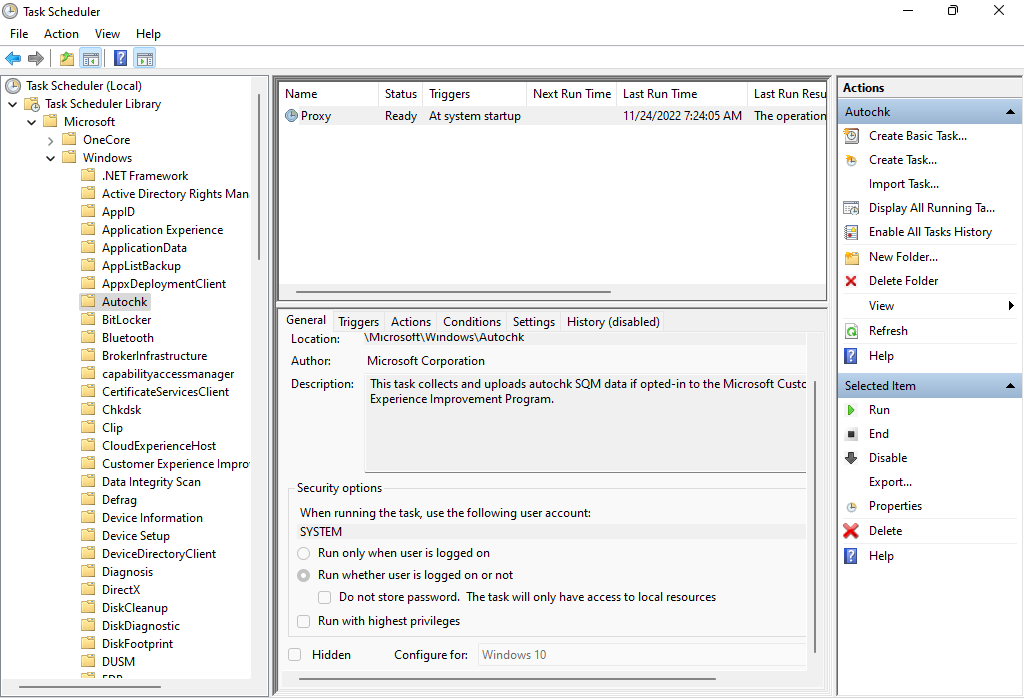
\includegraphics[width=\textwidth]{attacks/neither/05_taskscheduler_autochk.png}

% edit with start cmd.exe and trigger manually
% whoami
We can modfiy the action it performs to run our payload instead, to verify the privieleges our payload is executed with, we can save the output of the \lstinline{whoami} into a file. The \lstinline{whoami} command shows the current user and privileges \cite{windows-whoami}. After manually triggering the task we see that our payload was run from the \lstinline{nt authority\system} user account, which is the most privileged system account \cite{microsoft-localsystem-account}.

% chntpw and reged
% edit Task in machine under Control
We can export this modified registry key and as part of our attack import it on our victim's system. To import the key we can use a linux utility called chntpw whose primary purpose it is to reset the password of local windows user accounts \cite{chntpw}. The library does this by editing the registry of a Windows installation and as such the author also offers a standalone registry editor called reged.

% test
% dual boot
We can test the Linux tool when dualbooting a Linux and a Windows installation. We place our payload in the Windows installation and then boot into Linux, where we can simply open the \lstinline{HKEY_LOCAL_MACHINE/SOFTWARE} hive with reged and import our modified registry key.
% import and override registry key on target machine
This overrides the executable path of task's action and when booting into Windows our payload is now executed.


% port to uefi
The next step is to port the reged utiliy so that it works in the UEFI environment as a DXE driver, that our rootkit can interact with. We will call this driver RegedDxe from now on.
% most stdlib stuff is just mapping to UEFIlib stuff with equivalents or using gcc implementations
This process boils down to providing semantically equivalent definitions of external function calls, such as c standard library and Linux kernel functions, to link against. Declarations and macros are still supplied by the local compiler's system headers. Definitions can often be translated to UEFI equivalents, EDK2 has libraries offering implementations of commonly used abstraction.
% memory allocation (malloc, calloc, realloc), memory manipulation (memset, memcpy) string manipulation (sscanf, strtol), stdout (printf), abort, exit
Memory allocation maps to the MemoryAllocationLib, memory manipulation to BaseMemoryLib, basic string manipulation to BaseLib, stdout to PrintLib (only relevant for print debugging).

% cstdio is non trivial and has to be implemented by calling protocols on the right volume
Function calls related to standard input and output such as opening, reading and writing a file, namely the hive file, are more complex and have to be mapped to UEFI protocols like \lstinline{SimpleFileSystemProtocol} and \lstinline{FileProtocol}.

\TODO{no need to change reged source code}

RegedDxe unlike the original linux utility reged is not an application that is executed within a working directory, it is instead a DXE driver offering a protocol for other drivers to call.

% reged protocol
% The process to tackle this is by first isolating the functionality that is demanded by the regist driver, this is done through designing the protocol with which our main rootkit will interact with. The protocol is very simple, we only need a single function that imports a registry key into a hive.


% modify so that registry key can differ and found via matching values
When importing a registry key the target path for the key is read from the registry key file, cached task's registry keys do not follow a strict naming sheme and are instead named by GUIDs, thus they may differ from device to device. To combat this, we change the import mechanism, so that instead of importing a key into its exact path it iterates over the children of the target's parent key. We can then match for our target key with a value that correctly identifies the target key, such as the value representing the path of the XML, that was initially used to load the task.






